\documentclass[a4paper,12pt,headsepline]{report}

%----------------- PDF CONFIG ----------------- %
\pdfinfo{    
     /Title (PDF-Titel) 
     /Subject   (PDF-Thema)    
     /Author  (Vorname Nachname) 
     /Keywords   (Stichwort1,Stichwort2)      
} 

\title{MyTitle}
\author{theAuthor}
\date{1.1.2000}



%----------------- PAKETE INKLUDIEREN ----------------- %

\usepackage{geometry} % Packet für Seitenrandabständex und Einstellung für Seitenränder
\usepackage[ngerman]{babel} % deutsche Silbentrennung

\usepackage{booktabs} %entzerrt die Tabellenzeilen und bietet verschieden dicke Unterteilungslinien
\usepackage{longtable} % Tabellen können sich nicht über mehrere Seiten 
\usepackage{graphicx} % kann LaTeX Grafiken einbinden

\usepackage[applemac]{inputenc} % Umlaute unter Mac werden automatisch gesetzt
\usepackage[T1]{fontenc} % Zeichenencoding
\usepackage{lmodern} % typographische Qualität 
\frenchspacing % Schaltet den zusätzlichen Zwischenraum ab
\usepackage{fix-cm}
\usepackage{hyperref} % verwandelt alle Kapitelüberschriften, Verweise aufs Literaturverzeichnis und andere Querverweise in PDF-Hyperlinks
\usepackage{color}
\usepackage{url}


\usepackage[nottoc]{tocbibind}



% für Listings
\usepackage{listings}
\lstset{numbers=left, numberstyle=\tiny, numbersep=5pt, stepnumber=4, keywordstyle=\color{black}\bfseries\itshape, stringstyle=\ttfamily,showstringspaces=false,basicstyle=\footnotesize,captionpos=b}
\lstset{language=java}



%----------------- FARBEN DEFINIEREN ----------------- %
\definecolor{gray}{gray}{0.95} % Listingsbackground

%----------------- LAYOUT SETZEN ----------------- %
\geometry{left=2cm, right=2cm, top=2.5cm, bottom=2cm}
\linespread {1.25}\selectfont %1.25 da er von Haus aus 1.2 ist und 1,25 * 1,2 = 1,5 isch




%-------##-------##-------##------- ANFANG INHALT -------##-------##-------##-------%
\begin{document}



\pagenumbering{roman} % Seitennummer

%----------------- DECKBLATT -----------------%
 %----------------- KONFIGURATION ----------------- %
\pagestyle{empty} % enthalten keinerlei Kopf oder Fuß 

%----------------- HDA FBI Logo ----------------- %
\begin{figure}[t]
	\centering
	
\includegraphics[width=0.6\textwidth]{Abb/logo_fbi}
\end{figure}

%----------------- INHALT ----------------- %

\begin{center}
\Large Hochschule Darmstadt \\
\normalsize \textsc{- Fachbereich Informatik -} \\

% Whitespace
\vspace{105 pt}

\Huge Name der Arbeit \\ 
\normalsize
\vspace{20 pt}

Abschlussarbeit zur Erlangung des akademischen Grades \\ 
Bachelor of Science (B.Sc.) 

\vspace{75 pt}


vorgelegt von \\
\vspace{5 pt}
Can Kedik \\
731620
\vspace{115 pt}

\begin{tabular}[h]{p{4cm}l l}
	Referent: & Prof. Dr. Ronald C. Moore\\
	Korreferent: & Prof. Dr. Bettina Harriehausen-M"uhlbauer
\end{tabular}


\end{center}

 
%----------------- ABSTRACT -----------------%
 %----------------- KONFIGURATION ----------------- %
\pagestyle{empty} % enthalten keinerlei Kopf oder Fuß


\chapter*{Abstract} % (fold)
\label{cha:abtract}
	Lorem ipsum dolor sit amet, consetetur sadipscing elitr, sed diam nonumy eirmod tempor invidunt ut labore et dolore magna aliquyam erat, sed diam voluptua. At vero eos et accusam et justo duo dolores et ea rebum. Stet clita kasd gubergren, no sea takimata sanctus est Lorem ipsum dolor sit amet. Lorem ipsum dolor sit amet, consetetur sadipscing elitr, sed diam nonumy eirmod tempor invidunt ut labore et dolore magna aliquyam erat, sed diam voluptua. At vero eos et accusam et justo duo dolores et ea rebum. Stet clita kasd gubergren, no sea takimata sanctus est Lorem ipsum dolor sit amet.

\begin{quote}
Dies ist ein Zitat.
\end{quote}

verstand, scheinen nun doch vorueber zu Dies ist der Text sein. \\
siehe: http://janeden.net/die-praeambel

 
 
%----------------- VERZEICHNISSE -----------------%
\tableofcontents % Inhaltverzeichnis

% ----- Abbildungen ----- %
%\addcontentsline{toc}{section}{Abbildungsverzeichnis} % falls in Inhalsverzeichnis
\listoffigures

% ----- Tabellen----- %
% \addcontentsline{toc}{section}{Tabellenverzeichnis}  % falls in Inhalsverzeichnis
% \fancyhead[L]{Abbildungsverzeichnis / Abkürzungsverzeichnis} %Kopfzeile links
\listoftables

% ----- Listings ----- %
% Listingverzeichnis soll im Inhaltsverzeichnis auftauchen
% \addcontentsline{toc}{section}{Listingverzeichnis}
% \fancyhead[L]{Abbildungs- / Tabellen- / Listingverzeichnis} %Kopfzeile links
\renewcommand{\lstlistlistingname}{Listingverzeichnis}
\lstlistoflistings

\pagestyle{plain} % zurueck setzen von roemische seitenanzahl


%----------------- KAPITEL : EINFÜHRUNG  ----------------- %
\pagenumbering{arabic}
\chapter{Einf"uhrung}
\label{cha:einfuehrung}

Lorem ipsum dolor sit amet, consetetur sadipscing elitr, sed diam nonumy eirmod tempor invidunt ut labore et dolore magna aliquyam erat, sed diam voluptua. At vero eos et accusam et justo duo dolores et ea rebum. Stet clita kasd gubergren, no sea takimata sanctus est Lorem ipsum dolor sit amet. Lorem ipsum dolor sit amet, consetetur sadipscing elitr, sed diam nonumy eirmod tempor invidunt ut labore et dolore magna aliquyam erat, sed diam voluptua. At vero eos et accusam et justo duo dolores et ea rebum. Stet clita kasd gubergren, no sea takimata sanctus est Lorem ipsum dolor sit amet.



%----------------- KAPITEL : GRUNDLAGEN  ----------------- %	
\chapter{Grundlagen}
\label{cha:grundlagen}

Lorem ipsum dolor sit amet, consetetur sadipscing elitr, sed diam nonumy eirmod tempor invidunt ut labore et dolore magna aliquyam erat, sed diam voluptua. At vero eos et accusam et justo duo dolores et ea rebum. Stet clita kasd gubergren, no sea takimata sanctus est Lorem ipsum dolor sit amet. Lorem ipsum dolor sit amet, consetetur sadipscing elitr, sed diam nonumy eirmod tempor invidunt ut labore et dolore magna aliquyam erat, sed diam voluptua. At vero eos et accusam et justo duo dolores et ea rebum. Stet clita kasd gubergren, no sea takimata sanctus est Lorem ipsum dolor sit amet.

	
%----------------- KAPITEL : FAZIT  ----------------- %	


\chapter{Fazit}
\label{cha:fazit}

Lorem ipsum dolor sit amet, consetetur sadipscing elitr, sed diam nonumy eirmod tempor invidunt ut labore et dolore magna aliquyam erat, sed diam voluptua. At vero eos et accusam et justo duo dolores et ea rebum. Stet clita kasd gubergren, no sea takimata sanctus est

	\section{Unterpunkt} % (fold)
	\label{sec:unterpunkt}
		Lorem ipsum dolor sit amet. Lorem ipsum dolor sit amet, consetetur sadipscing elitr, sed diam nonumy eirmod tempor invidunt ut labore et dolore magna aliquyam erat, sed diam voluptua. At vero eos et accusam et justo duo dolores et ea rebum. Stet clita kasd gubergren, no sea takimata sanctus est Lorem ipsum dolor sit amet.
	% section unterpunkt (end)
	



%----------------- KAPITEL : BEISPIELE  ----------------- %	
\chapter{Beispiele}
\label{cha:beispiele}
	Dieses Kapitel soll viele alltaegliche Beispiele\footnote{Fussnote} abdecken um einen {\LaTeX} Dokument zu setzen

		\section{Schriftarten}
		\label{sec:schriftarten} 
			\begin{itemize}
				\item Kursiv: \emph{Das ist ein Beispiel}
				\item Unterstreichen: \underline{Das ist ein Beispiel}
				\item Fettschrift: \textbf{Das ist ein Beispiel}
				\begin{itemize} 
					\item Kombination aus dreien: \underline{\textbf{\emph{Das ist ein Beispiel}}}						\end{itemize} 
				\item Serifen: \textsf{Das ist ein Beispiel}
				\item Schreibmaschinen Schrift: \texttt{Das ist ein Beispiel}
				\item Kleine Grossbuchstassen: \textsc{Das ist ein Beispiel}
				\item Ausfuehrungszeichen: ``Das ist ein Beispiel''
				\item asld
			\end{itemize}
			
		
			\subsection{Symbole}
				\begin{enumerate}
				\item Deutsche Umlaute: "A, "O, "U, "a, "o, "u, "s
				\item Sammlung von Sonderzeichen \url{http://de.wikibooks.org/wiki/LaTeX-Kompendium:_Sonderzeichen}
				\end{enumerate}
				

	\section{Abbildungen}
		Wie folgt bindet man Abbildungen ein:
		% Beispiel für Bildintegration
		\begin{figure}[htb]
		 \centering
		 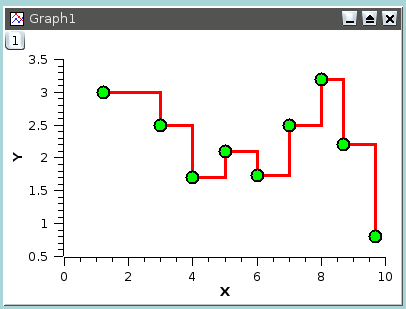
\includegraphics[width=0.4\textwidth,angle=0]{Abb/beispiel}
 		\caption{Beispiel Bild; Quelle ist png}
		\label{fig:beispiel}
		\end{figure}
	
	\section{Tabellen}
			Lorem ipsum dolor sit amet, consetetur sadipscing elitr, sed diam nonumy eirmod tempor invidunt ut labore et dolore magna aliquyam erat, sed diam voluptua. At vero eos et accusam et justo duo dolores et ea rebum. Stet clita kasd gubergren.

		\begin{center}
			\begin{tabular}{lcrc} \toprule
			Stadium & Substratfreie Kontrolle  & \multicolumn{2}{c}{Probenansatz} \\\cmidrule(rl){3-4}
			 & Farbe & Farbe & Bewertung \\\midrule
			Alpha1 & farblos & braun & +++ \\
			Beta2 & farblos & farblos & - \\\bottomrule 
			 \end{tabular}
		 \end{center}
		 
		2. Beispiel \\
		\begin{table}[h]
		\centering	 
		 	\begin{tabular}{|l|l|c|}
			\hline
			\textsc{Rang} & \textsc{Name} & \textsc{Rating}\\
			\hline
			\hline
			1 & Garry Kasparov & 2817\\
			2 & Viswanathan Anand & 2774\\
			3 & Wladimir Kramnik & 2764\\
			\hline
			\end{tabular}
		\caption{Beispiel Beschriftung einer Tabelle}
		\label{tab:beispiel}
		\end{table}
		
		


	\section{Verweise}
		Hier werden Verweise auf verschiedene Elemente erstellt \cite{lin1973}
		\subsection{Pageref und Ref} 
			Diese Textstelle ist sehr interessant.\label{interessant} \\				
			Hier wird auf die Textstelle~\ref{interessant} verwiesen, \\
			die sich auf der Seite~\pageref{interessant} befindet.\\[20pt] 
			Verweis auf Listing \ref{lst:javaBsp} auf Seite \pageref{lst:javaBsp} \\
			Verweis auf Abbildung \ref{fig:beispiel} auf Seite \pageref{fig:beispiel} \\
			Verweis auf Tabelle \ref{tab:beispiel} auf Seite \pageref{tab:beispiel}
			
	\section{Listing}
		\lstset{language=java}
		\begin{lstlisting}[frame=hl, caption={Das Listing zeigt Java Quellcode} ,backgroundcolor=\color{gray}, label={lst:javaBsp}]
/* Java Hallo World Beispiel */

public class HelloWorld {
    public static void main(String[] args) {
        System.out.println("Hello, World");
    }
}
		\end{lstlisting} 
		
	
\nocite{wiki:xxx}
\bibliographystyle{amsalpha}
\bibliography{literatur}
\pagenumbering{Roman}	
	

	
\end{document}
